\chapter{Holistic Approach to Modular Open Educational Resources for Computer Graphics\label{chap:ExGoer}} %Florian Diller, Text from Fabian
In recent years, the \acrfull{oer}~\cite{wiley:2014:oer} as well as \acrfull{cg} has continued to grow. Hence, in this chapter, we present a holistic modular approach to experiential \acrshort{cg} education as \acrshort{oer}.

Although many computer graphics applications such as video games, 3D data visualization, and animated movies have existed for several decades, they still continue to gain importance. A German national survey conducted in 2023 found that 36 percent of youths aged 12 to 19 played video games every day~\cite{jim:2023:studies}. 
The worldwide revenue generated by the gaming industry of 249.44 billion \acrshort{usd} in 2023 emphasizes its significant economic importance~\cite{Statista-Market-Insights:2023:Videogames-worldwide}. The corresponding employment opportunities highlight how important goal-driven computer graphics education is in preparing new graduates with the skills and knowledge necessary to take on challenges and opportunities in gaming, visualization, and other related fields. Since 1983, increasing numbers of research projects have examined and analyzed the growing importance of \acrshort{cg} education~\cite{Balreira:2017:topics-cg-teaching}.

Suselo~\cite{Suselo:2019:problems-cg-teaching} examines the range of subjects needed to instruct students in computer graphics. These cover a wide range of basic concepts from various fields, including physics, mathematics, and programming. Additionally, grasping geometric concepts requires the ability to envision these concepts in a three-dimensional space. For example, Lui~\cite{Lui:2022:problems-cg-teaching} discovered that 3D imagination positively correlated with \acrshort{cg} test scores and programming test scores. However, \acrshort{cg} is mostly explained using traditional teaching techniques and media, which convey difficult \acrshort{cg} concepts through static 2D representations. As a result, learners must tackle the additional challenge of raising the content to a new, higher level of abstraction to understand it.

%\section{Previous Work on CG Learning\label{sec:previous}} %Fabian Pueschel
Despite the promising applications that have been created in the past, the availability to students and educators is often very limited, resulting in the described \acrshort{cg} learning environments being insufficient or not available for teaching purposes. In this chapter, we propose a holistic, goal-oriented approach to teaching mathematical-visual concepts and providing them sustainably in the form of \acrshort{oer}. The teaching materials presented here are inspired by the pedagogical framework presented by Püschel et al.~\cite{pueschel:2013:MRCG}, who have adapted Kolb's model of the experiential learning cycle~\cite{kolb:1984:experiential} to meet the challenges of modern \acrshort{cg} teaching. The main objective is the shaping and reflection of the learning experience with the help of educational modules (see \autoref{fig:contents}) consisting of classical lecture slides, interactive applications ("exploratories"), and additional learning process monitoring.

In contrast to Püschel's study~\cite{pueschel:2013:MRCG}, our research has comprehensively analyzed the optimization of the three teaching components mentioned above in line with the \acrshort{oer} concept and their public availability in a sustainable way. Our work covers the inter-institutional usage of lecture slides and quizzes in learning management systems, as well as the creation and usage of 14 interactive \acrshort{cg} web applications for different \acrshort{cg} topics. Previous findings on \acrshort{cg} learning environments are integrated into learning applications with the means of a game engine, providing students with a user-friendly interface with in-app challenges and explanations, as well as illustratory and exploratory parts. We call this experiential learning applications \emph{exploratories}, referring to Van Dam~\cite{vanDam:1999:education}, who created the term as a combination of \emph{exploratorium} and \emph{laboratory}, describing computer-based applications for experimentation and investigation. In addition to an exploratory, each educational module contains slides explaining the theory and a quiz for evaluating testing learning successes as visualized in~\autoref{fig:contents}.

\begin{figure}[b!th]
	\centering
	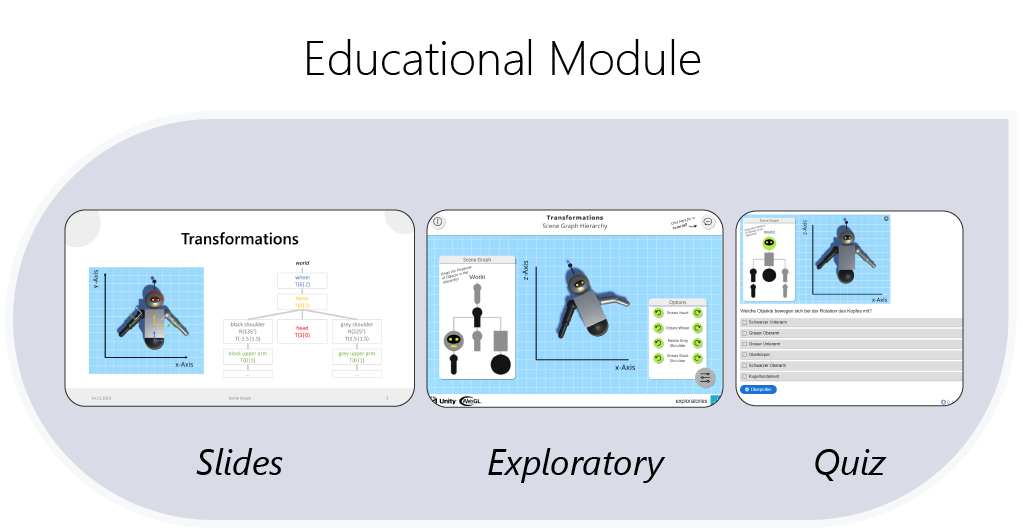
\includegraphics[width=0.8\linewidth]{pictures/ExGoerContents.png}
	\captionsetup{labelfont=bf,textfont=it}
	\caption[Contents of educational modules.]{Each of our educational modules consists of an exploratory, slides, and a quiz.\label{fig:contents}}
\end{figure}


\section{Related Work} %Fabian Pueschel
To facilitate the learning of \acrshort{cg} for students, the intrinsically visual subject areas of \acrshort{cg} were recognized as early as 1999~\cite{Balreira:2017:topics-cg-teaching}, and the resulting recommendations for interactive \acrshort{cg} learning applications were highlighted. These have recently been the subject of several scientific publications, and the resulting learning applications can be categorized into programming-based and conceptual approaches:

\textbf{Programming-based approaches}, utilize code or parameters to visually modify computer graphics themes. They can make use of software libraries like \emph{Three.js} or WebGL~\cite{angel:2017:interactive} or simplified programming environments~\cite{Sueyasu:2010:cg-tool},~\cite{Lobb:2016:cg-tool}. While Angel~\cite{angel:2017:interactive} uses \emph{Three.js} and WebGL to teach \acrshort{cg} simultaneously with an awareness of web programming, tools like "Simplified Language for Graphics Programming" (SLGP) and "CodeRunnerGL" offer less complicated environments for teaching rendering and 3D animations using pseudo-code~\cite{Sueyasu:2010:cg-tool},~\cite{Lobb:2016:cg-tool}.

\textbf{Conceptual learning settings} usually concentrate on teaching complex topics either by conveying the fundamental ideas step-by-step or not at all. These belong to the category of \emph{top-down} teaching approaches, which have been used for instance, in computer graphics, to teach different camera systems and transformations without assuming or exploring complex principles of mathematics or programming. This approach to teaching computer graphics is increasingly common in the current literature~\cite{Suselo:2019:problems-cg-teaching}. It is demonstrated through the creation of applications for personalized learning or using existing software.

Using \textbf{established software solutions} such as Maya~\cite{maya:2024:software} or Blender~\cite{blender:2024:documentation} modeling software, the software's internal functionalities are used to explain computer graphics concepts such as transformations, object creation, and animation~\cite{Elyan:2012:cg-tool},~\cite{Kadam:2013:cg-tool}. With this method, students can learn the functions and controls of the program while also comprehending three-dimensional representations more easily~\cite{Kadam:2013:cg-tool}. This enables students to understand the program more quickly while also understanding the notion of \acrshort{cg} in three dimensions. However, the teaching content is restricted to the built-in features of the program being used, and it can only be marginally modified to fit particular teaching methods. For this reason, it may be necessary to create dedicated learning apps to teach more specific subjects. Thus, the scientific literature on teaching particular \acrshort{cg} material frequently concentrates on the \textbf{creation of conceptual learning programs}, which can be downloaded or run locally on a desktop computer, or mobile, for instance, \acrfull{ar} apps.
Although there are apparent advantages of \acrshort{ar} in education~\cite{wu:2013:current}\cite{lilligreen:2019:AWI}\cite{lilligreen:2019:EuroVR}, \acrshort{ar} apps usually require mandatory installation~\cite{Qiao:2019:disadvantage-of-ar}, which makes consistent use during \acrshort{cg} lessons difficult. However, when implemented as a platform-independent web application, the advantage arises that all students have constant access to the latest version of the application and it can be opened through a variety of output media without the need for installation~\cite{Eisemann:2023:cg-tool},~\cite{angel:2017:interactive}.  This is one of the reasons why our educational modules contain interactive web applications for the \emph {experiential learning} aspect.


Despite the variety of learning environments, the resulting learning platforms share many similarities in their forms of \textbf{interaction and topics}. To facilitate comprehension of complex \acrshort{cg} concepts without engaging in the theoretical basics, the complexity is often reduced by using predefined interfaces in the spirit of \emph{conceptual learning settings}. In addition to predefined interfaces, our educational modules go a step further and strive to not only provide consistent ways of interactions across different topics but also to have a consistent look and feel. For this purpose, all modules are built using the same foundational framework of templates developed throughout the work of our study.

Predefined interfaces are frequently used to reduce complexity in \acrshort{cg} concepts so that they can be comprehended more easily without requiring an in-depth knowledge of theory. The "Graphic Teaching Tool" by Spalter and Tenneson~\cite{Spalter:2006:cg-tool} focuses on parameter-based modification of scenes and their visual representation. It adapts different graphics pipelines and their special features, such as transformations, and visualizes the resulting matrices using the example of the local desktop application. Further research has focused on different visualization and interaction approaches for teaching ray tracing processes~\cite{Suselo:2018:cg-tool},~\cite{ Verschoore-de-la-Houssaije:2022:cg-tool}, as well as the rendering pipeline, camera movements, and shadow mapping~\cite{Eisemann:2023:cg-tool}. Some of these topics are also covered by our set of \acrshort{oer} modules (see~\autoref{sec:topics}) and the remaining can be easily developed based on the presented foundational framework.

There is a growing body of literature regarding \textbf{\acrfull{oer}} as presented by Wiley et al.~\cite{wiley:2014:oer}. Regarding \acrshort{cg}, the Computer Graphics Educational Materials Source (CGEMS) as described in Figueiredo et al.~\cite{figueiredo:2003:cgems}, \cite{figueiredo:2004:cgems2} as well as Anderson et al.~\cite{anderson:2017:NewCGEMS}, of the ACM SIGGRAPH Education Committee and Eurographics Education Board offer educational \acrshort{cg} materials licensed under Creative Commons. Additionally, Ridge and Terzopolos~\cite{ridge:2019:ecosystem} introduced an online encyclopedia for computer graphics resources. Much like our work, it conveys different aspects of learning and combines them in a repository. Furthermore, it is possible to view some real-time animation examples within the encyclopedia. Like Wikipedia, it is to be seen rather as a work of reference. However, our education modules are specifically created with teaching \acrshort{cg} in mind as a consistent package of ready-to-use materials. %https://github.com/encyclopedia-of-code/tiny-graphics-js
%https://www.realtimerendering.com/basics3js


\section{OER - Terminology and Challenges \label{sec:challenges}} %Florian Diller
As Wiley et al.~\cite{wiley:2014:oer} stated, there are a variety of definitions for the term \acrshort{oer}. In our work, we refer to the \emph{Paris Declaration} of 2012~\cite{declaration:2012:paris}, which uses the definition of the term from \acrshort{unesco}’s 2002 Forum on Open Courseware.

Atkins et al.~\cite{atkins:2007:review} already pointed out several challenges for \acrshort{oer} to overcome in 2007, which were revisited seven years later by Wiley et al.~\cite{wiley:2014:oer}. In 2021  Tlili et al.~\cite{tlili:2021:towards} name the following challenges that \acrshort{oer} face:
\begin{itemize}
	\setlength{\itemsep}{-0.3cm}
	\item Lack of innovative teaching strategies
	\item Difficulty in monitoring the learning process
	\item Searching and locating \acrshort{oer}
	\item Mapping \acrshort{oer} together
	\item Feedback
	\item Adaptive learning
	\item Protecting intellectual property
	\item Fraud prevention
\end{itemize}

While we do not intend to solve these issues with the chapter at hand, there are some aspects, that are linked to these challenges.

\section{Topics Overview\label{sec:topics}}
%Listing of all exploratories and SHORT description
As already mentioned before, we developed educational modules for 14 different \acrshort{cg} topics. To give the readers an impression of the context for which we developed the foundational framework and holistic integration we list the realized modules in the following. We also provide a short description of the exploratory contents of each module.
\begin{enumerate}
	\setlength{\itemsep}{-0.3cm}
	\item \textbf{Scene Graph:} Example scene with interactive scene graph hierarchy and interactive objects (visible in the middle of~\autoref{fig:contents})
	\item \textbf{Light Sources:} Scene with different variable light sources
	\item \textbf{DDA Line Drawing:} Educational game, where the user has to place pixels similarly to a line drawing algorithm (see \autoref{fig:uxEval}a)
	\item \textbf{Field of View:} Example scenes with interactive viewing frusta to see the impact of the parameters in real-time (see \autoref{fig:uxEval}b)
	\item \textbf{Occlusion Culling:} Interactive example of occlusion culling and frustum culling with an overview to visualize the appearing and disappearing of objects
	\item \textbf{Backface Culling:} Different scenes including an interactive camera, an object with color-coding of culled faces, as well as displayed calculation
	\item \textbf{Level of Detail:} Moving the camera replaces different objects with more or less detailed counterparts depending on distance
	\item \textbf{Shading:} Examples of different shading methods with a variable light source, level of detail, and reflections
	\item \textbf{Transformations:} Editable transformation matrix featuring highlighting regions responsible for  rotation, scaling, and translation, and an object visualizing the respective transformation
	\item \textbf{2D Curves:} Hermite and B{\'e}zier curves with interactive boundary conditions and displayed basis matrix
	\item \textbf{Rotation:} Successively executable breakdown of the rotation around an arbitrary axis with variable axis location and rotation angle (see \autoref{fig:uxEval}c)
	\item \textbf{Convolution:} Step-wise executable convolution with variable filter sizes and padding options
	\item \textbf{Subdivision:} Step-wise animated execution of several iterations of the Catmull-Clark subdivision in 2D and 3D
	\item \textbf{Mesh Simplification:} Animated example of a grid-based mesh simplification algorithm with clickable cells allowing to initiate specific simplification steps
\end{enumerate}
All modules are publicly available as described in~\autoref{sec:publication}.

\section{Holistic Approach}
In this section, we describe the details of the design and development of our educational modules. As mentioned before, they each include an application, presentation slides, and a quiz (see~\autoref{fig:contents}), and each of the modules is focused on a specific topic. Key features of the educational modules include consistency, modularity, and expandability to ensure a coherent and customizable learning and teaching experience. The following section systematically introduces these features, providing brief explanations of their relevance to our work, followed by a more detailed exploration in subsequent sub-sections, clarifying where these features manifest within the implementation, educational modules, in-app tasks, and challenges.

As a tool for the development of the exploratories, the game engine Unity~\cite{unity:2024:editor} has been chosen. Creating template scenes and templates objects (called \emph{prefabs} in Unity's terminology) for use with the game engine, we provide a modular framework that enables the creation of customized learning experiences through the seamless integration of pre-built components. In addition, various tools are made available to the user to facilitate the creation of personalized applications, supported by extensive documentation explaining technical aspects and guidelines.

\textbf{Consistency:}
Consistency serves as the backbone of our comprehensive approach, seamlessly linking all elements within our three-part modules. In the modules, including applications, presentations, and quizzes, uniform utilization of images, graphics, and textual content is used to facilitate a cohesive and integrated learning experience. The intuitive consistency promotes a holistic approach to understanding computer graphics and related areas, supporting a fluid and engaging learning journey.

\textbf{Modularity:}
Modularity is a foundational element in our approach, allowing the creation of independent, self-contained learning units. These units consist of modules encompassing an application, presentation slides, and a quiz. Furthermore, in the development of individual applications using our framework, multiple development templates can be employed. Yet, combined they form a rich learning experience. Each module stands on its own and allows students to focus on specific topics. This not only facilitates focused learning but also allows instructors to adapt and expand individual modules to meet the specific needs of their students, promoting flexibility and individualization.

\textbf{Expandability:}
Expandability is an essential part of our intention to create continuous improvement and adaptability. The following aspects establish easy expansion and updating: The open-source character of our \acrshort{oer} combined with the modular approach in development, extensive documentation, annotation of the provided templates, the use of freely editable file formats (e.g. H5P~\cite{Singleton_Charlton_2019} for quizzes), and the use of a development environment (here game engine) in widespread use. This ensures that our content remains dynamic and offers educators the opportunity to improve existing modules or create new ones as technology and with it educational needs evolve. This adaptability contributes to the longevity and relevance of our educational resources.

\begin{figure}[h!tb]
	\centering
	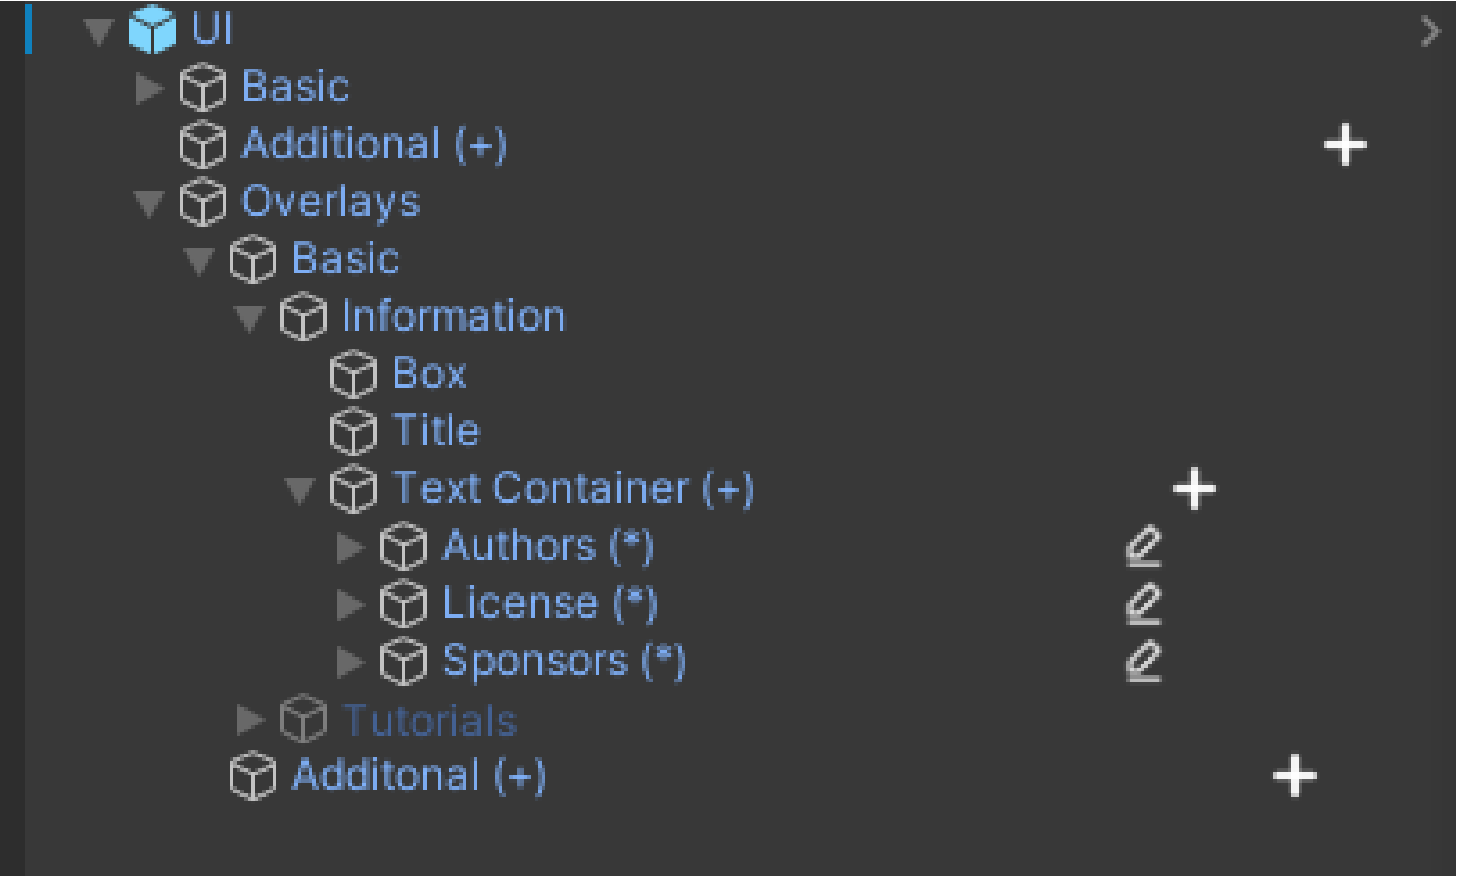
\includegraphics[width=0.6\linewidth]{pictures/userGuidance_Icons.png}
	\captionsetup{labelfont=bf,textfont=it}
	\caption[Icons indicate user interaction.]{The icons in the scene hierarchy let the user quickly identify possibilities to contribute. The \emph{pen} icon indicates editable objects, the \emph{plus} icon marks where new objects can be added.\label{fig:userGuidance}}
\end{figure}

\textbf{User Guidance:}
Icons (see~\autoref{fig:userGuidance}) and documentation in the provided templates make it clear where the resources can be used and adapted effectively. This user guidance is designed to help teachers and developers make changes exactly where they are needed without unnecessary complications. This guided tailoring of resources to individual needs increases the accessibility, usability, and overall effectiveness of our education system.

These key aspects collectively represent the concept of our overall design, which is not only technologically sophisticated but --- more importantly --- learning process-oriented. They form the backbone of an ecosystem where connectivity, adaptability, and accessibility come together to create a dynamic and enriching learning and teaching experience for students and teachers alike.


\subsection{Implementation}
%\textcolor{blue}{Modular., Expand, User Guidance (UI)} How do the above key points show in the implementation?

Our application comes with a framework of prefabs and scenes in the game engine Unity that follows a modular design approach. These components can be flexibly combined to create different applications within the educational package as visualized in \autoref{fig:unityPrefabs}. The provided Unity scenes are easy to use for certain control types. For example, developers can choose between a 2D or a 3D scene that is already equipped with the appropriate controls, user interface (UI), and camera. In addition, the provided prefabs make it easier to expand the UI by enabling the integration of useful elements such as buttons or tutorials. This modular structure not only increases the adaptability of the package but also facilitates the creation of customized educational experiences.
The pre-built UI is designed to support additional features to meet different educational needs. Users can easily expand the UI with features such as buttons and panels, providing a platform for the creation of advanced and customized learning applications.
Cues within the Unity framework, such as icons for editable or extensible components in the \emph{hierarchy}, provide clear visual guidance for user interaction (see~\autoref{fig:userGuidance}). These indicators, combined with detailed technical information presented in the comprehensive documentation, allow users, i.e. developers, to navigate the development environment with confidence.

\begin{figure}[h!tb]
	\centering
	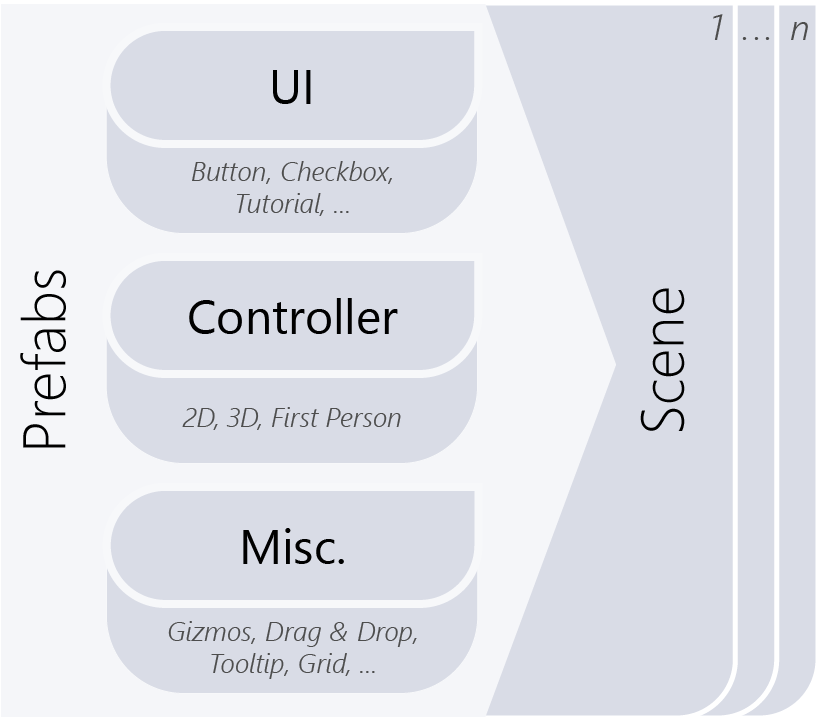
\includegraphics[width=0.6\linewidth]{pictures/unityPrefabs.png}
	\captionsetup{labelfont=bf,textfont=it}
	\caption[Structure of educational templates.]{Template objects (so-called \emph{prefabs}) enable the user to easily create customized scenes fit for their needs. \label{fig:unityPrefabs}}
\end{figure}

\subsection{Educational Modules} %Teaching Bundles?
%\textcolor{blue}{Interconn., Modular (Folien,Quiz), Expand (Educational), User Guidance (Docu)} How does the above key points show in the framework?
The digital educational content has been carefully designed to flow seamlessly together and ensure a consistent visual identity. Each exploratory includes multiple recognizable graphical elements and details that reappear in the presentation slides and H5P quiz modules, creating a cohesive look and feel that enhances understanding of the topic. This can be seen, for example, in the screenshots of \autoref{fig:contents}.
The concept of modularity and expandability in our project is manifested through the deliberate design of multiple self-contained topics. Each learning unit operates as an independent module. This design allows for seamless integration and interchangeability of these units within an overall educational framework, e.g. in a lecture as visualized in \autoref{fig:modularApproach}. Whether educators wish to modify the sequence, introduce new content, or adapt existing modules, the modularity and expandability of our project allow them to do so effortlessly. This approach not only enhances the adaptability of the educational content but also facilitates a dynamic learning environment where each unit serves as a building block for teaching material fitting the educators' needs and a learning experience tailored to individual student groups. In addition, the widespread formats of the educational materials enable effortless integration within existing learning management systems (in our test scenarios, \emph{Moodle} and \emph{OLAT} were used) to deploy them among students and to evaluate the learning progress.
\begin{figure*}[h!bt]
	\centering
	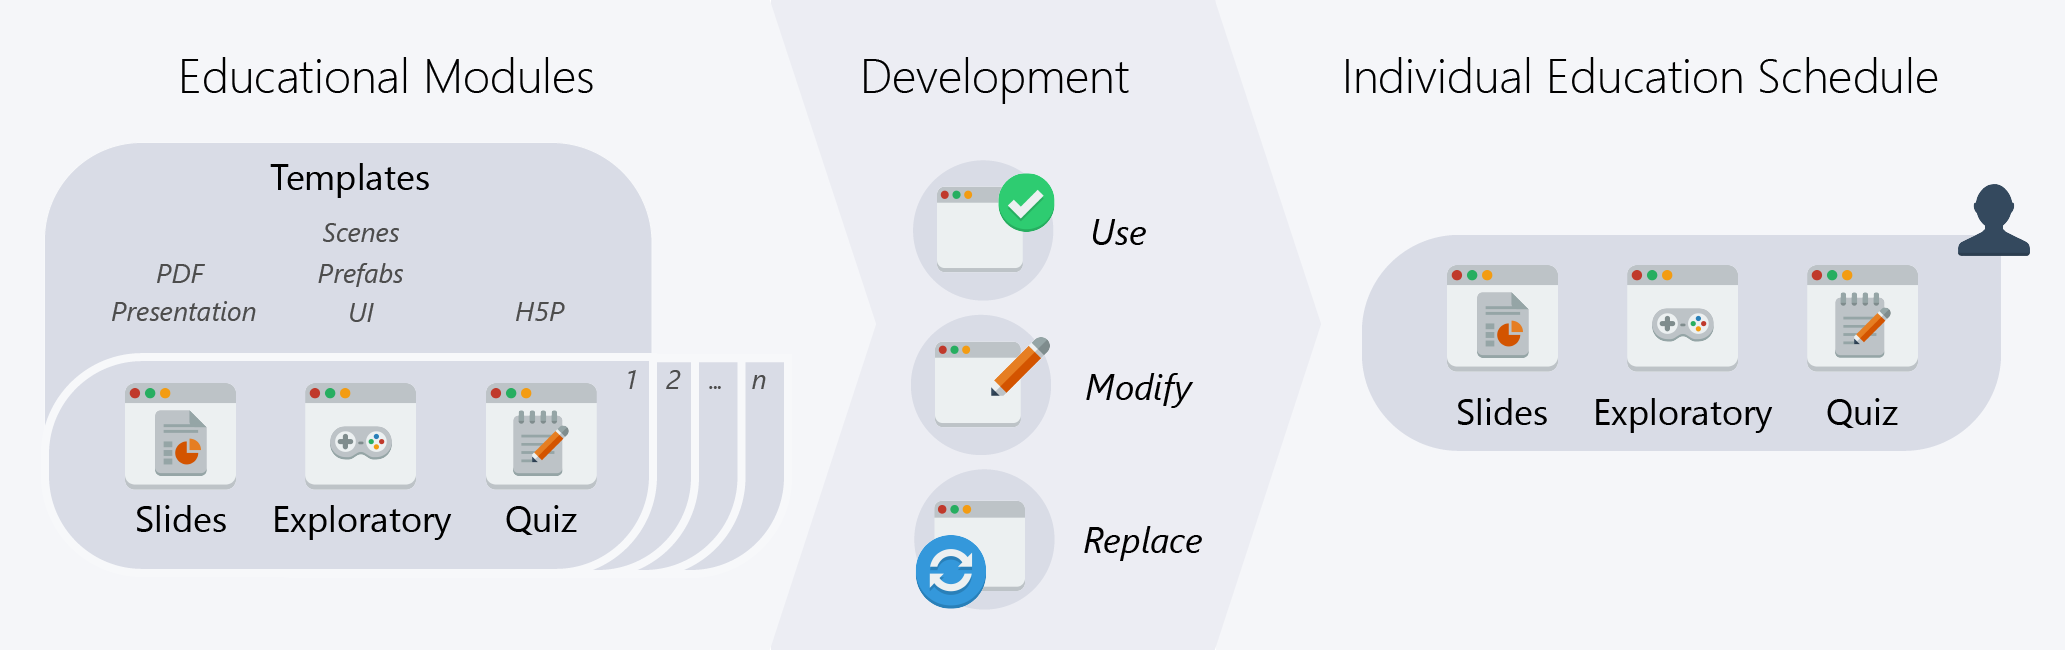
\includegraphics[width=\linewidth]{pictures/modularApproach.png}
	\captionsetup{labelfont=bf,textfont=it}
	\caption[Systematic overview of the educational approach.]{Systematic overview of our educational approach and how to implement it in education schedules. We provide $n=14$ modules that are based on shared templates, which give them a consistent look and feel. By using the templates to create new modules, reusing or modifying existing modules, or replacing parts, other educators can create their own modules tailored to their individual teaching schedules.\label{fig:modularApproach}}
\end{figure*}
\subsection{In-App Tasks and Challenges}
%\textcolor{blue}{exploratories zum erkunden (FOV, Transform), gamification (DDA)}
In-app tasks serve as catalysts for active learning. These tasks are designed to motivate students to delve deeper into the subject matter and encourage them to apply theoretical concepts in a hands-on environment. By linking theoretical learning with practical tasks, we aim to promote a deeper understanding of the content. Another approach taken by us is inspired by gamification, bringing elements of competition and achievement into the learning process (see e.g. subfigure~\ref{fig:DDA}).
%The tasks in the app are designed not only as assessments but also as exciting challenges that transform the learning process into a quest for knowledge and insight.
This gamification approach not only increases motivation but also fosters a sense of accomplishment as students successfully complete each challenge. The integration of in-app tasks and challenges aligns seamlessly with our broader educational design philosophy. These challenges are intentionally chosen to align with specific learning modules, ensuring a direct connection between theoretical concepts presented in slides and applications and their practical use in the challenges. As students progress through the challenges, they not only reinforce their understanding of theoretical knowledge but also gain enthusiasm for exploration.

In summary, our holistic approach allows us to provide a cohesive, adaptable, and user-friendly learning experience. The incorporation of consistency, modularity, expandability, and user guidance forms a versatile foundation. Moreover, the integration of in-app tasks and challenges elevates the learning experience, turning it into an engaging process for both teachers and learners.

Our learning modules are available on the project website (\href{https://openedu-rlp.de/edu-sharing/components/collections?id=fd3957ef-80aa-4440-8956-c1d0d738c629}{https://www.openedu-rlp.de}). It includes the materials needed for forming individual learning schedules as seen in~\autoref{fig:modularApproach}. Additionally, there can be found the source files and documentation to use and build upon our materials, or create new exploratories. Furthermore, the materials can be found via other services, which refer to the project website. %The repository is publicly available at \url{https://gitlab.rlp.net/exgoer/exploratories.git}. 

\section{Evaluation}
%The integration of Open Educational Resources (OER) into education has earned increased attention in recent years, aligning with the ongoing trend of making educational content more open and accessible.
The following subsections describe the three different methods how we evaluated our newly developed overall concept and the specific educational modules. The aim is not only to assess the effectiveness of this concept and the modules but also to examine its pedagogical significance and potential challenges for educators and learners alike. The first two subsections explore the expert knowledge of a small number of individuals, while the third subsection provides insights into the interaction with a larger number of learners.

\captionsetup{labelfont={bf,color=black},textfont=it}
\begin{figure*}[h!tb]
	\centering
	\subfloat[DDA Line Drawing\label{fig:DDA}]{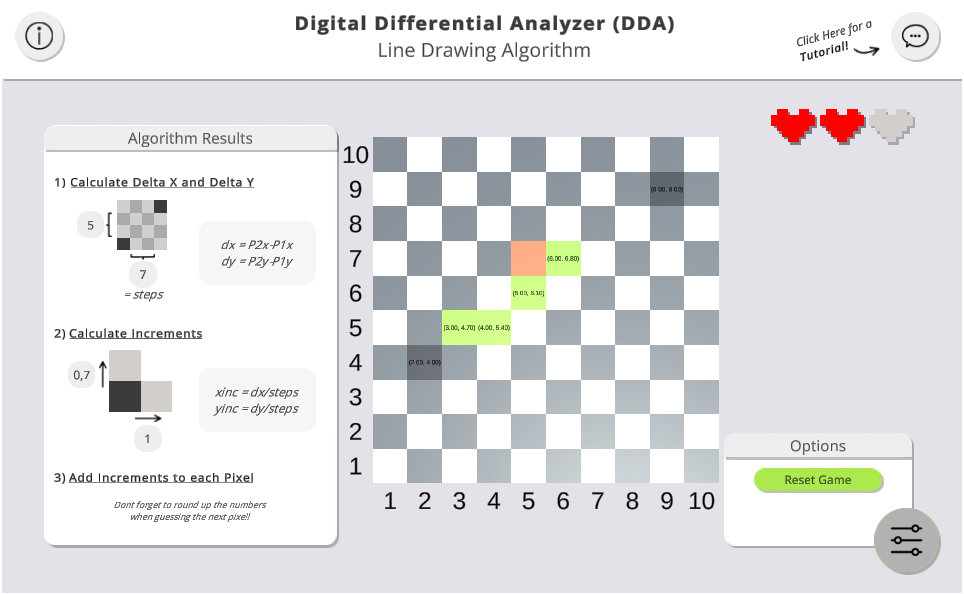
\includegraphics[width=0.33\linewidth]{pictures/DDAScreen.png}\hfill}
	\subfloat[Field of View]{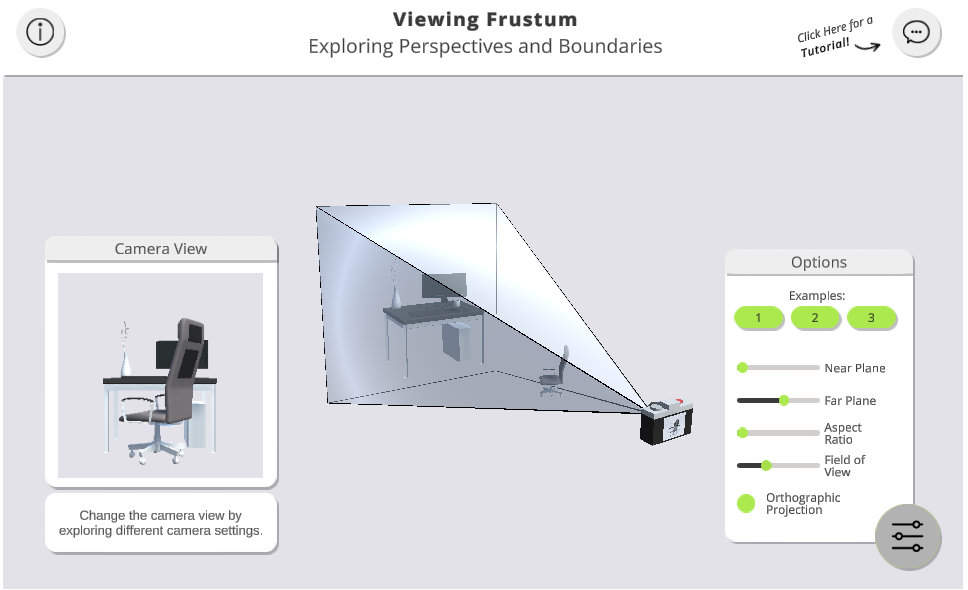
\includegraphics[width=0.33\linewidth]{pictures/fovScreen.png}\hfill}
	\subfloat[Rotation]{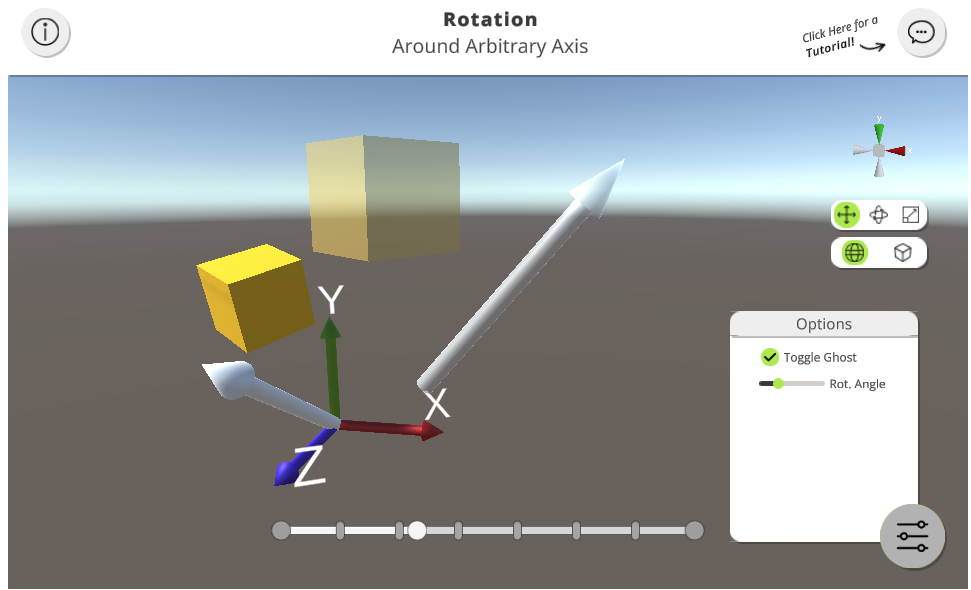
\includegraphics[width=0.33\linewidth]{pictures/RotationScreen.png}\hfill}
	\captionsetup{labelfont=bf,textfont=it}
	\caption[Screenshots of user evaluated exploratories.]{Screenshots of the selection of exploratories used to evaluate the UX of our modules. This should provide an overview of the contents and the design. The panels on the left provide additional information, and the panels on the right offer options to manipulate the scene.}
	\label{fig:uxEval}
\end{figure*}
\section{Publication\label{sec:publication}}

\subsection{Teaching Staff Interviews}%Julian Stockemer
This subsection examines the willingness to use the concept and the impact of its integration on teaching practice. This survey, involving five participants, was conducted during a university event focused on \acrshort{oer}. The participants were introduced to our teaching concept, had the opportunity to experience the exploratories \emph{Field of View}, \emph{Backface Culling}, and \emph{Light Sources}, and posed questions. Subsequently, they completed a questionnaire.
The purpose of the survey was to obtain feedback from both educators and external participants. The questionnaire began by asking about the current integration of external tools and openness to interactive teaching methods. Following this, participants evaluated the utility of the presented concept in teaching and expressed their willingness to incorporate it into their lectures. Additionally, their inclination to utilize the provided examples developed by us or adapt the template for their own instructional content was queried. If respondents encountered challenges in these aspects, they were encouraged to list them.

Our teaching concept is primarily aimed at teachers and students. Nonetheless, we sought input from external participants to identify possible perspectives outside the educational community. Among the participants, three out of five were active in teaching. Four of five participants expressed a readiness to adapt their methods, with most of them integrating external content regularly. The unanimous desire for more interactive elements underscores their perceived pedagogical value.
In addition, another four of five participants were open to adopting the presented teaching concept, though half noted a need for additional skills for effective implementation. Despite this, all participants agreed on the content's accessibility and its meaningful contribution to student learning.
In summary, educators showed a positive inclination toward integrating interactive elements, with openness to the presented concept. The unanimous consensus on the accessibility of content provides a promising basis for the widespread adaption and adoption of the \acrshort{oer} modules we presented.


\subsection{UX-Design Expert} %Florian Diller
To ensure the quality of our work concerning usability, a selection of three exploratories (\emph{DDA Line Drawing}, \emph{Field of View}, and \emph{Rotation}) as seen in~\autoref{fig:uxEval} with the corresponding slides was given to a UX design expert. Subsequently, a questionnaire with different statements was answered. Its results will be presented in the following.

The UI was predominantly good to use with no inconsistencies. Furthermore, it seemed to the expert that most users would quickly learn to handle the educational modules. The modules seemed rather straightforward and the integration of various functions in the system appeared successful. However, the navigation through the application would profit from a more detailed explanation. Especially one exploratory stood out, which was difficult to understand without the proper inclusion in a lecture. Although applications themselves feature a tutorial, they are intended to be included in a lecture and properly introduced by an instructor, which we were not able to provide to the UX-design expert. %Nevertheless, we see the module in question as a chance for further improvement.

The overall impression of our educational modules was highly attractive to the UX design expert.

\subsection{Students} % Florian Diller
We evaluated our experiential approach in practice by implementing eight exploratories in lectures. The selection consisted of the topics \textit{Transformation}, \textit{Rotation}, \textit{Scene Graph}, \textit{Shading}, \textit{Light Sources}, \textit{2D Curves}, \textit{Subdivision}, and \textit{Mesh Simplification}. The students took part in the experiments voluntarily.

To evaluate our approach among students, we applied split testing involving 19 individuals. Both randomized groups listened to a lecture regarding the educational content at hand. Subsequently, a quiz was taken by each participant. Then one group repeated the content with the conventional learning method of reviewing the script of the lecture heard. The other group followed the experiential approach and worked with the exploratory. Finally, both groups took the same quiz again and we recorded the increase of correct answers. Thus we were able to assess if the use of our exploratories leads to a larger improvement than conventional repetition methods. Overall, the improvement was evaluated 79 times across different exploratories. In our study, instructors did not explain the exploratories to the students in order to make the results of the study independent of the influence of individual instructors. The educational effect of the exploratories, however, could be improved by the instructor introducing the exploratories in detail.

The group of students using the exploratories showed a slightly higher improvement in test scores, 18~\% on average, than the group using conventional slide reading, which improved by 11~\% on average. When looking at the results, we see that some participants scored 100~\% in the first and second try, which leads to an improvement of 0~\%. Because these participants did not have the chance to improve at all, we could ignore them to get a clearer understanding of the improvement. Doing so, we see an average improvement of 25~\% in the group with the exploratories compared to 17~\% improvement in the group with slides. However, by conducting a one-tailed t-test with \(\ \alpha=0.05\), we see no statistical significance, considering the p-values of \(p=0.2>\alpha\) and \(p=0.16>\alpha\) with the data cleaned like explained above.
Nevertheless, the students responded exclusively positively to the exploratories and quizzes when conducting the experiments. For instance, the students requested permanent access to the exploratories and quizzes to support their studies. Furthermore, students expressed that the exploratories helped them understand the subject better, as the exploratories showed a different approach to it and let them experience the learning contents.

%possibly add "insights/discussion" section

\section{Conclusion} %Florian Diller
As the amount of \acrshort{oer} is constantly growing, accessibility and fairness of education are raised. Consequently, education is made available to an increasing number of people from various cultures and backgrounds.

In this chapter, we presented a novel holistic modular approach to \acrshort{oer}. We developed educational modules for 14 \acrshort{cg} topics and published them as well as evaluated them with various user groups. The responses were positive throughout. While the evaluation of exploratory impact showed no statistical significance, a positive tendency was visible. The opinions we gathered from students, educators, and professionals showed that the use, development, and teaching of our \acrshort{oer} modules appealed to them.

As mentioned in~\autoref{sec:challenges}, the challenges \acrshort{oer} face are a topic, which is regularly revisited. Tlili et al.~\cite{tlili:2021:towards} mention several. Our work might represent a first step in solving some of them. The \emph{lack of innovative teaching strategies}, for instance, is addressed by the holistic experiential learning approach of our three-part education modules. The use of quizzes and exploratories activates the students and introduces variety to classrooms and lecture halls. Furthermore, the quizzes make it easier to \emph{monitor the learning process} and the platform on which we published our work allows for referencing from other websites, which simplifies \emph{searching and locating \acrshort{oer}}.



\section{Future Work}
Although the chapter at hand showed a comprehensive way to develop, publish, and use \acrshort{oer} packages, there are still desirable developments for the future. For instance, the framework we created will be used as a base to expand the existing topics and broaden the variety of exploratories and materials. Furthermore, the game engine we employed to develop the framework and the exploratories presented in this chapter is free of charge in certain situations (e.g. \acrshort{oer}), but we intend to migrate the application framework to an open-source game engine like Godot (\url{https://godotengine.org/}) because it lines up even further with the ideas of \acrshort{oer} to use open-source software to develop and access our materials. Additionally, our approach represents a good foundation for implementing \emph{microcredentials}. Following this approach, smaller educational topics are formally certified. This might raise the relevance of the project even further, make it possible to interlink it with other educational programs, and provide verifiability. Lastly, the impact of our work should be further assessed to a statistical significance. Consequently, we plan on conducting a more extensive user study.